\documentclass[11pt]{article}
\usepackage{amsmath}
\usepackage{enumitem}
\usepackage{fullpage}
\usepackage{geometry}
\usepackage{graphicx}
\usepackage{array}


\usepackage[colorlinks=true, allcolors=blue]{hyperref}
\usepackage[utf8]{inputenc}


% Support for easy cross-referencing
\usepackage[capitalize]{cleveref}

\geometry{top=1in, bottom=1in, left=1in, right=1in}

\newcommand{\code}[1]{{\small \tt #1}}


\title{CS 393R Autonomous Robots \\ \large Project}
\author{Elvin Yang, Jierui Lin, Aidan Dunlap}
\date{December 10, 2021}

\begin{document}
\maketitle

%%%%%%%%%%%%%%%%%%%%%%%%%%%%%%%%%%%%%%%%
\section{Introduction}

\begin{figure}[t]
\begin{center}
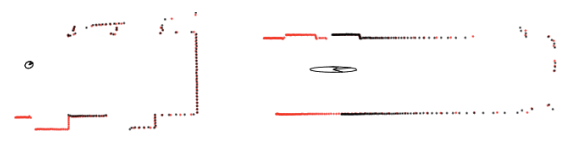
\includegraphics[width=\linewidth]{hallway.png}
\end{center}
\caption{In the left environment, position is well constrained while the long hallway in the right figure lacks longitudinal constraints, so that the estimation is uncertain in that direction.
}
\label{fig:teaser}
\end{figure}
Simultaneous localization and mapping (SLAM) is a popular algorithm for deploying mobile robots, and the
performance of SLAM systems often depends on the environment.
For example, in a rank-deficient environment, such as a long hallway, there is high uncertainty in a certain direction due to lack of features to constrain the search space, yielding inaccurate mapping and localization. 

To tackle this problem, robust rank-deficient SLAM~\cite{Nashed2021RobustRD} is proposed to use larger features to find correspondence. More specifically, they extract lines from observation point clouds and use those to establish correspondences between observations. Such feature is very suitable for regular, man-made environments and can increase localization and mapping accuracy while being more robust to outliers.

In order to quantitatively evaluate the method's performance, we follow~\cite{Kmmerle2009OnMT} to compare the relative displacement error of our prediction compared with the recorded data.




\section{Algorithms}

\subsection{Feature Detection}

To extract line segments from laser scans, we implement a modified version of the iterative end-point fit algorithm (IEPF).
Our implementation of IEPF tries to fit a line segment to a sequence of points using the endpoints of the sequence, rejecting the line if any of the following conditions are not satisfied:

\begin{enumerate}
    \item The number of points in the sequence is less than a threshold.
    \item The length of the line segment is below a threshold.
    \item The distance between any pair of successive points is above a threshold.
    \item The distance from any point in the sequence to the line is above a threshold.
\end{enumerate}

\noindent
If all conditions are satisfied, the line segment formed by the endpoints of the sequence is considered valid.
If all conditions except the last are satisfied, the sequence is split into two about the point with maximum distance to the line segment. The process is repeated until all sequences of points have been processed.
The initial sequence of points is sorted in increasing scan angle of the corresponding laser scans from the LIDAR sensor.

\subsubsection{IEPF Hyperparameters}

We use the following hyperparameters for the IEPF conditions.

\begin{enumerate}
    \item Minimum points per line segment: 9
    \item Minimum line segment length: 0.2 meters
    \item Maximum distance between successive points: 1 meter
    \item Maximum allowable point distance from the line segment: 0.1 meters
\end{enumerate}

\noindent
Since most environments are not completely linear and have some amount of noise, we tuned these parameters to extract relatively large and dense features. We found that the setting for the first two hyperparameters filter out small clusters of points formed by environmental noise like footsteps and furniture legs. The third hyperparameter mainly prevents the algorithm from fitting a line to sparse noise. We assumed a real standard deviation of about 5 centimeters for the LIDAR sensor. In the datasets we used for tuning, setting the final hyperparameter to 10 centimeters seemed to keep a good balance between keeping large features and breaking line segments for corners and curves in the environment.

\subsection{Cost Function}

To establish correspondences between line segment features, we use a modified version of the line segment similarity metric proposed in ``Robust Rank-Deficient SLAM''\cite{Nashed2021RobustRD}.

$$C(a, b) = ((\alpha\ d_\theta)^2 + d_\bot^2 + d_\parallel^2)^\frac{1}{2}$$

where 
\begin{itemize}
    \item $d_\theta$ is the $\sin$ of the angle between the two line segments as vectors
    \item $d_\bot$ is the perpendicular distance between the centers of the line segments
    \item $d_\parallel$ is the minimum distance between the endpoints of $b$ to $a$ when projected onto $a$
\end{itemize}

The number of line segments extracted from a laser scan is typically small ($< 20$), allowing us to perform naive correspondence matching by sorting the set of all possible correspondences between successive sets of line segments. To limit false correspondences we only consider pairs with a cost less than 3.

\subsubsection{Hyperparameters}

We added a hyperparameter $\alpha$ to the $d_\theta$ term since $\sin(\theta) \approx \theta$ for small $\theta$. We define $\alpha = 3 * (l_{\max} / l_{\min})$. The ratio of line lengths serves to discourage correspondences between lines with very different lengths.

\subsection{Evaluating Accuracy}
''On Measuring the Accuracy of SLAM Algorithms''\cite{Kmmerle2009OnMT} proposes a novel way for evaluating SLAM algorithms that overcomes deficiencies in prior techniques. The paper identifies classical techniques of evaluating SLAM accuracy by comparing absolute position points, notably the temporal position of a misprediction. The paper identifies the main classical technique as 


$$\varepsilon\left(x_{1: T}\right)=\sum_{t=1}^{T}\left(x_{t} \ominus x_{t}^{*}\right)^{2}$$

\begin{center}
    where $a \ominus b$ be the transformation to get from a to $b$. 
\end{center} 

With this technique, a displacement mismeasure at the start of an evaluation session will propagate to the end and show up in every time step past the hour, all summed up at the end. On the contrary, a same displacement mismeasure at the end of a sequence will only include the delta of the last point, differing from the prior sequence, with practically the same error, by an integer factor.  

Rather than this technique, the authors propose a simple formula that overcomes this propagation error by observing the deltas between points and comparing them to ground truth data. The authors propose 

$$\text { Let } \delta_{i, j} \text { be } x_{i} \ominus x_{j}\text{. } \varepsilon(\delta)=\frac{1}{N} \sum_{i, j} \operatorname{trans}\left(\delta_{i, j} \ominus \delta_{i, j}^{*}\right)^{2}+\operatorname{rot}\left(\delta_{i, j} \ominus \delta_{i, j}^{*}\right)^{2}$$

This technique, comparing deltas between points, overcomes the propagation problem by looking at point pairs on a timestep by timestep basis, meaning an error in one prediction will not impact future ones down the line.

\section{Challenges}

Unfortunately, due to time constraints and a general unfamiliarity with the library, we were not able to get Ceres-Solver to converge in our SLAM backend. Instead of performing full optimization, we perform a local search around odometry-reported displacements, similar to correlative scan matching. However, instead of maximizing probabilities using rasterized maps, we minimize the cost function between established line segment correspondences.

\section{Experiments and Results}

We evaluate the performance of Correlative Scan Matching and our modified Rank-Deficient SLAM implementation using the MIT Killian Court dataset, ACES Building dataset, and metricEvaluator software provided by ~\cite{Kmmerle2009OnMT}. We truncate the datasets to 10 minutes.


% m{${x}em} means x em for column width
\begin{center}
\begin{tabular}{|l|c|c|}
\hline
\textbf{Dataset and Algorithm} & \textbf{Translational Error} & \textbf{Rotational Error} \\ 
\hline
Killian (RD-SLAM) & 0.49          & 0.07       \\ \hline
Killian (CSM)     & 0.50          & 0.07       \\ \hline
ACES (RD-SLAM)    & 0.25          & 0.11       \\ \hline
ACES (CSM)        & 0.26          & 0.11       \\ \hline
\end{tabular}
\end{center}

The mean error data output by metricEvaluator\cite{Kmmerle2009OnMT} is very similar between the two SLAM implementations. While this was somewhat expected since we were unable to perform full pose-graph optimization, looking at qualitative results (\ref{fig:csm}, \ref{fig:rdslam}) provides insights about differences between point-based and line-based approaches. We observe that the point-based approach has significant angular drift over time in the long hallway section of the Killian Court dataset, but preserves the structure of the map relatively well when making corner turns. In contrast, the line-based approach preserves the linear structure of the hallway very well, but struggles when making turns around corners. We hypothesize that occlusion effects prevent the extraction of meaningful line segments, reducing the number of established correspondences between scans. 

Naturally, we expect to see improved results in both approaches with full backend implementations. However, since we couldn't find detailed specifications about how the datasets we used were acquired, we made assumptions about characteristics like the sensor location in the base link frame and standard deviation of the sensor, which we think may have also contributed to inaccuracies in the generated maps.


\begin{figure}[p]
\caption{Killian Court Map (CSM)}
\centering
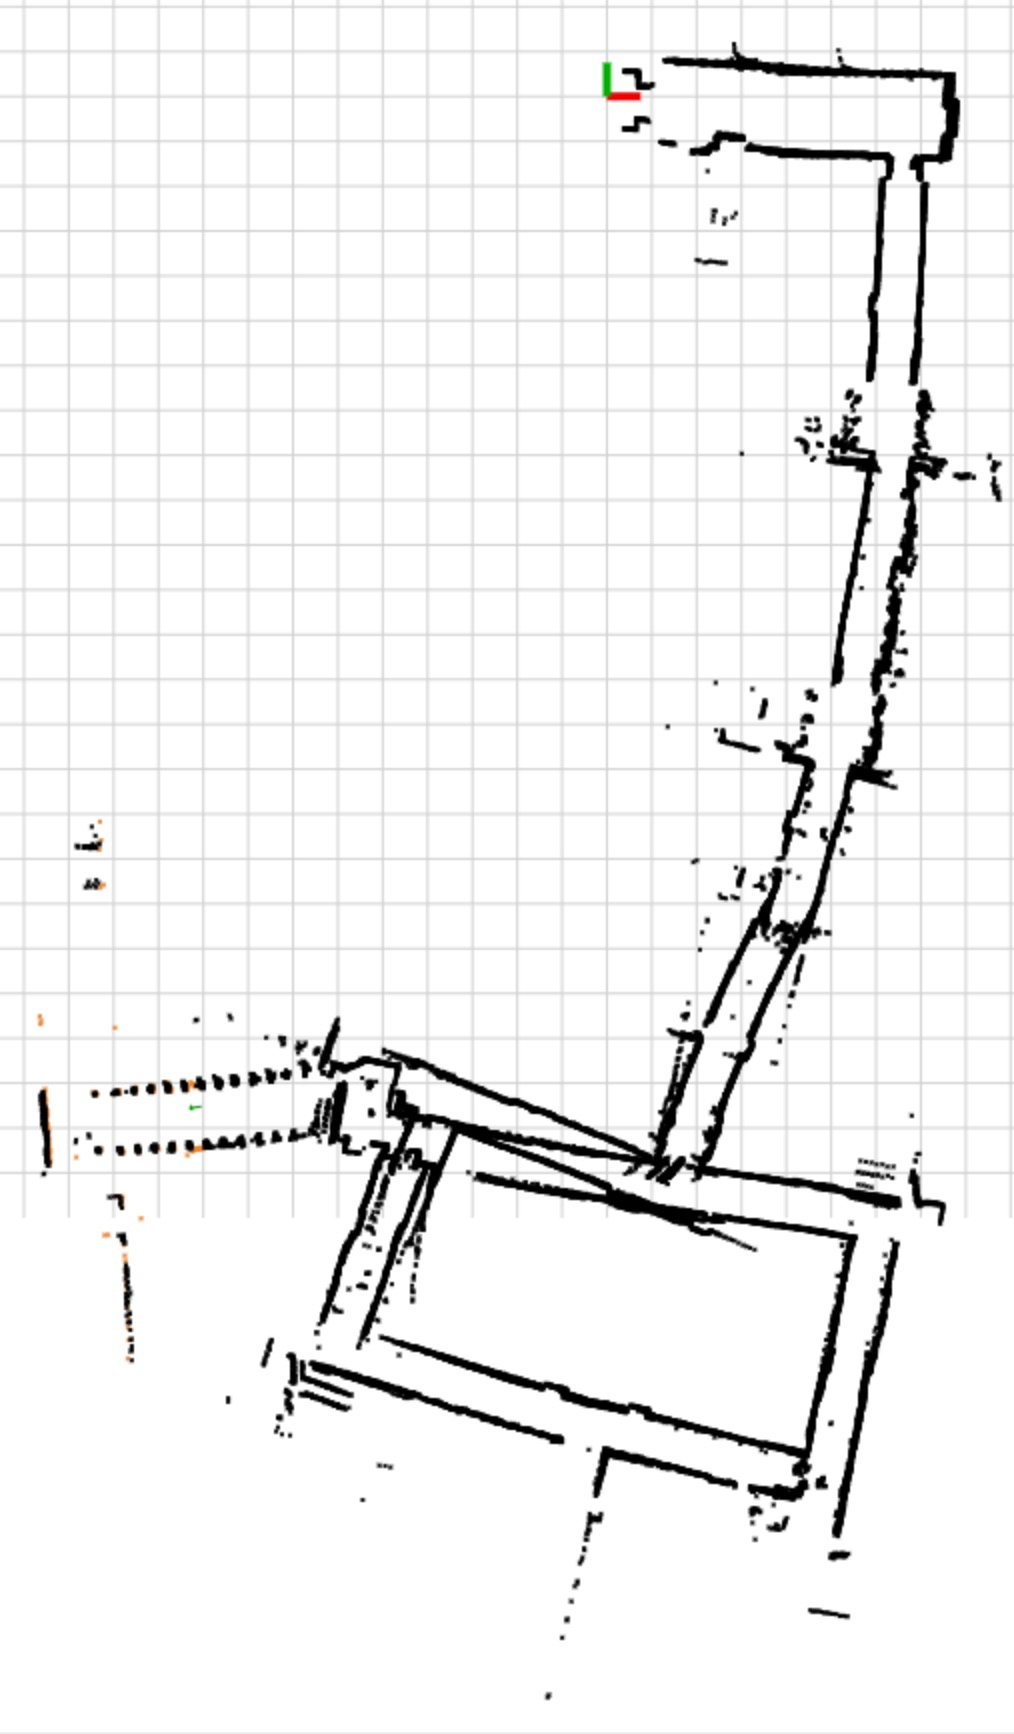
\includegraphics[height=8in]{csm-killian.jpg}
\label{fig:csm}
\end{figure}

\begin{figure}[p]
\caption{Killian Court Map (RD-SLAM)}
\centering
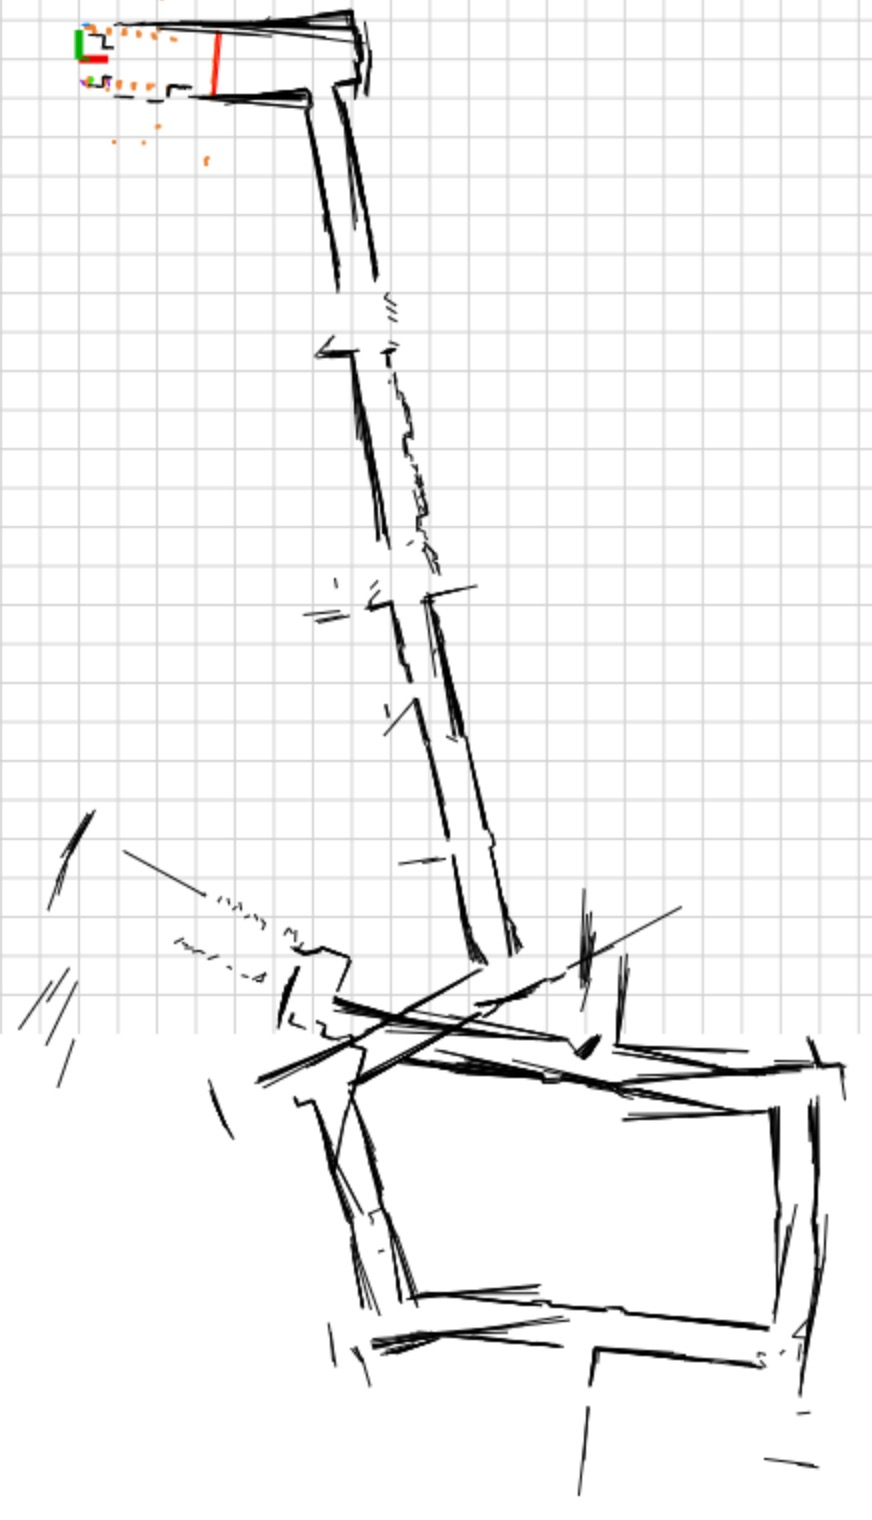
\includegraphics[height=8in]{rd-slam-killian.jpg}
\label{fig:rdslam}
\end{figure}

%%%%%%%%%%%%%%%%%%%%%%%%%%%%%%%%%%%%%%%%
\section{Repository Link}
\href{https://github.com/elvout/cs393r}{https://github.com/elvout/cs393r}


%%%%%%%%%%%%%%%%%%%%%%%%%%%%%%%%%%%%%%%%
\newpage
\appendix

\bibliographystyle{plain}
\bibliography{refs}


\end{document}
